% !TeX encoding = UTF-8

%\documentclass{LTHtwocol} % Use this when you work on your report.
 \documentclass[final]{LTHtwocol} % Use this for the final version.
                                   % It will remove page numbers and
                                   % markers for overfull boxes.
                                   % There really shouldn't be any of those anyway.

\usepackage[utf8]{inputenc}        
\usepackage{minted}
\usepackage{amsmath,amssymb,graphicx}

\usepackage{xcolor}
\usepackage{hyperref} 
\hypersetup{
	colorlinks,
	linkcolor={red!50!black},
	citecolor={blue!50!black},
	urlcolor={blue!80!black}
}




\addbibresource{bibliography.bib}


% Document begins here
\begin{document}
\begin{frontmatter}
\title{Portfolio Management of OMXS30 using Statistics and Deep Learning} % Title of the project.
                      % Note that all reports are in English,
                      %so that our international students can read them.

\author[måns]{Måns Sandsjö}
\author[august]{August Lindberg Brännström}

\email[måns]{ma8332sa-s@student.lu.se}
\email[august]{august.lindberg\_brannstrom.8120@student.lu.se}

\begin{abstract}
The goal of this project is to manage a portfolio of OMX Stockholm 30 stocks using Single-Period Optimization. This is done by collecting price data, cleaning it from outliers, predict future prices and covariance between the stocks and then optimize a portfolio based on this information. By using holding and trading constraints to solve a convex optimization problem, as formulated by Boyd et. al (2007) for each stock during each trading period, the portfolio is re-balanced with the predictions as parameters. How well the predicted returns and covariance are estimated for the model is measured by calculating the realized Sharpe ratio (SR) \& average turnover. Python is used as the main program for data handling and creating predictions. Initial portfolio management is made on simulated stock data and later on historical stock data is instead used during the years 2010-2020 of OMXS 30 closing prices. The methods used in the project to create predictions on future returns are simple moving average, exponential moving average and Long Short Term Memory whereas the covariance matrix in use is either sample covariance matrix or the covariance matrix as formulated by Ledoit \& Wolf (2004). With hyperparameter optimization the parameters are tuned to get the highest score regarding the metrics described above. The best performance achieved on the portfolio is a Sharpe ratio of 0.33 with corresponding average turnover of 23.25, more results will be discussed in the report. 

%    The abstract should be a 200--250 word compact description of your project. What was the objective? Which methods did you use? What was the (main) result?
\end{abstract}

\end{frontmatter}

% Stick to the proposed structure below. Add \subsections{} as appropriate.
% This file compiles on the Automatic Control Department system by typing the
% following into the terminal (while in the directory of the file, and with all
% other files belonging to the template untouched):
% > pdflatex template        
% > biber template
% The first line compiles the .tex file. The second line generates the
% bibliography. Once this is done, you may need to run the first line 1-2
% additional times, for the system to get all cross references right in the
% produced pdf output.

\section{Introduction}
The goal of this project is to manage an optimised portfolio of the 30 most traded stocks in Sweden, OMX stockholm 30, with the data provided from Investing.com \cite{ref:Investing}. This is done by collecting and evaluating data using holding and trading constraints as formulated by Boyd et. al (2007) using Single-Period Optimisation to solve a convex optimization problem between each given trade period\cite{Boyd}. All trading is simulated using real historical data in a backtesting environment. The result of the project can be seen in figure 1.

The project can be divided into three different sub-tasks:
\begin{itemize}
\item Data gathering \& cleaning
\item Build the convex optimization problem solver
\item Implement functions to create predictions on risk \& return
\end{itemize}

 

\begin{figure}[h]
	\centering
	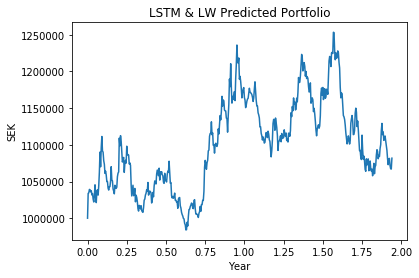
\includegraphics[width=0.8\columnwidth]{Pics/result/LSTM_LW.png}
	\caption{Total value of portfolio, using LSTM predicted returns and Ledoit \& Wolf estimated risk on OMXS30. Timespan is from 2018 to 2020.}
	\label{fig:LSTMLW} 
\end{figure}

%Here you introduce the project. What is the background? What project do you aim at solve? References to prior work? If the project makes a positive or negative environmental, or other solitary, impact, describe it here. Are there any ethical considerations? You might want to reference relevant literature, e.g. \cite{openclosed2, Hellerstein2004, Yun2015}. A general \LaTeX\ guide is available at \cite{latexwiki}. 

\subsection{Data gathering \& cleaning}
The data used is the open price on the stock market for each trading day on all the stocks in OMXS30 for the given time period. By cleaning the data from missing values/NaN-values \& outliers one can achieve a higher signal to noise ratio.

\subsection{Convex optimization problem}
%Förklara hur vi löser de konvexa optimeringsproblemet
Convex optimisation is a part within mathematical optimisation with many applications within areas such as finance and statistical analysis as well as automatic control systems, signal processing and more. With a set of constraint one is able to optimise a convex function to identify its maximum/minimum value highly efficient. To use convex optimization the function as well as the constraints, needs to be convex in their nature. This means that the local minimum/maximum in a convex function is equal to the global extrema. In comparison to non-convex optimisation-methods where one has to first identify multiple local extremum in order to then compare and conclude which of them are them are the global maximum/minimum and whether or not such a point exists. \cite{Boyd}

%Släng in en tydligare källa på detta

%Källa https://www.control.lth.se/fileadmin/control/Education/EngineeringProgram/FRTN50/Lectures/cvxfcn.pdf

%(source: https://web.stanford.edu/~boyd/cvxbook%/bv_cvxbook.pdf)

Convex optimisation is used for evaluating the fraction, hereby referred to as "weights", of each stock to be invested in for each given time period. The function accounts for the future return subtracted by the different cost and risk associated parameters. This is to be maximised and the outcome of the function is what weights should be used to produce the largest predicted risk adjusted outcome.\cite{Boyd}

\subsection{Predictions on risk \& return}
Initially, the predictions of future returns is estimated using simple moving average, referred to as SMA and exponentially weighted moving average, EMA. These are simple methods that works quite poorly as a mean of predicting the future returns, but they provide a basic understanding of the change of return-rate for a given time period. In practise they are rarely used for stock predictions. 

\subsubsection{Simple moving average} predictions are calculated as a moving average of returns from a specified amount of previous trading days. It evaluates the return rate from the previous trading days as equivalent, even if it is the return rate from the previous trading day or from the trading day two days ago etc. This method can be fine tuned based on how many historical returns that should be included.
\cite{ref:SMAEMA}

\subsubsection{Exponential moving average} predictions are exponantially weighted meaning that they are different from the SMA predictions in one way particular: the previous return rates are weighted different based on how many trading days ago they were current. This method can be fine tuned by changing a parameter that determines how much the historical returns should be accounted for. \cite{ref:SMAEMA}

\subsubsection{Risk} is estimated as the covariance of the return. In this project absolute risk is used, as described in Modeling, either based on the sample covariance matrix \cite{covar}, SCM, or as it is defined by Ledoit and Wolf (2004) \cite{Ledoit_Wolf}, LW. With SCM one can roughly  estimate the covariance of the assets with the rolling average of previous trading periods' covariance. LW is a more precise way of predicting the covariance matrix by using the previously implemented SCM and apply a transformation called "shrinkage" to it in order to reduce the estimation error. LW is therefore considered to be a more precise method of predicting covariance matrices with greater dimensions primarily when the amount of stocks are large in comparison to the amount of return data. 

\subsubsection{Long short term memory}  is the last method used to predict returns (hereby referred to as LSTM). LSTM is a neural network consisting of artificial neurons connected to each other. A neuron takes inputs and calculates outputs. By using weights, the neuron multiplies the inputs, makes a linear combination and lastly adds a constant. The neurons are then connected and layered. Multiple layers are used for a deep learning network. Through these layers the neural network learns the associations between inputs and outputs. \cite{uppsala} A structure of a two hidden layer neural network can be seen in figure \ref{fig:NN}.

\begin{figure}[h]
	\centering
	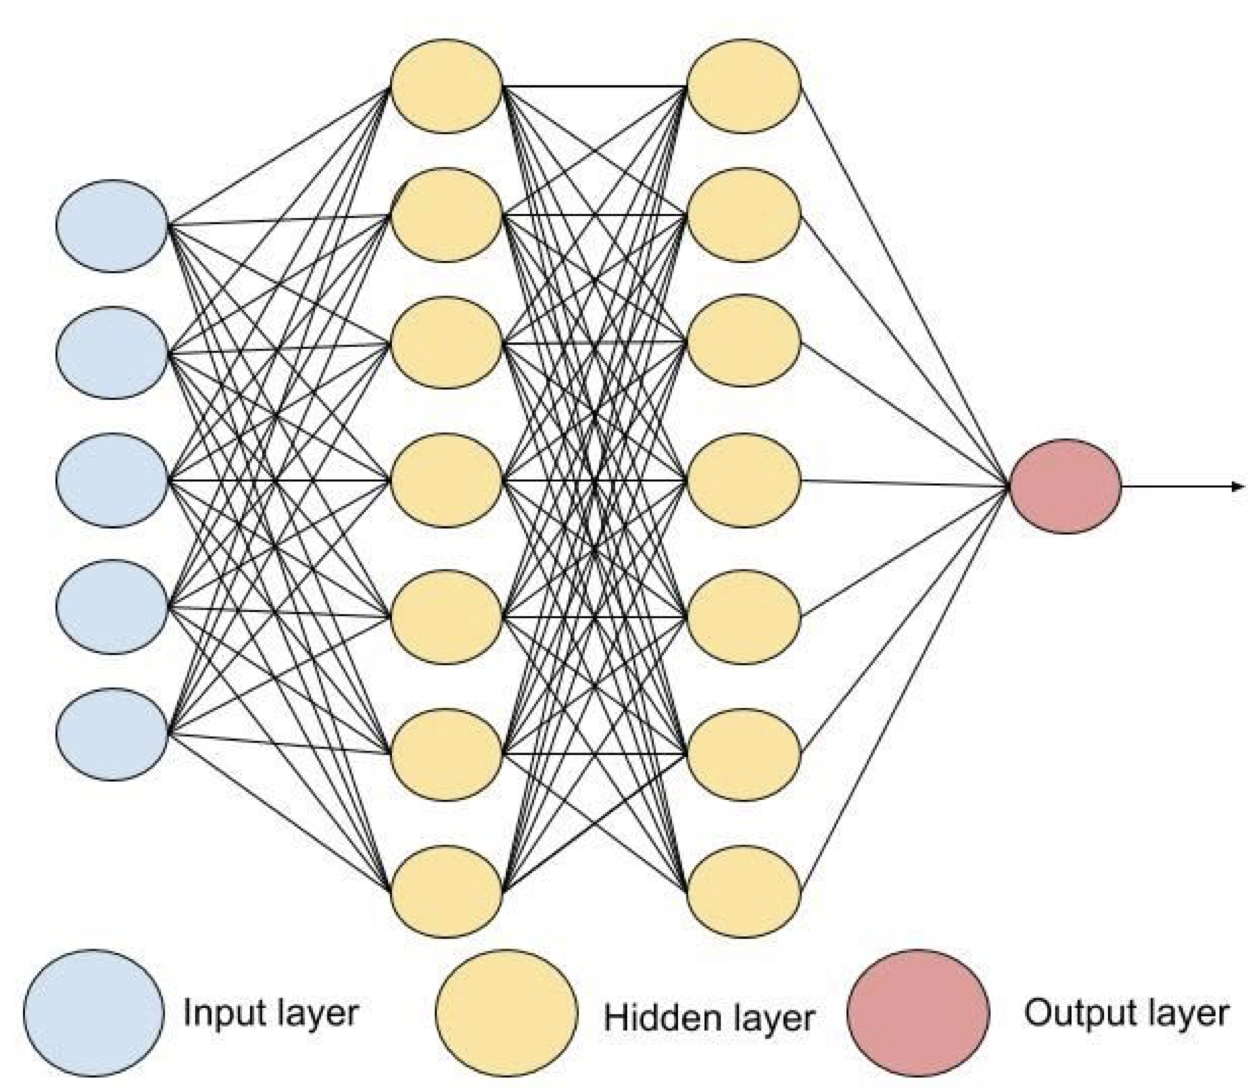
\includegraphics[width=0.7\columnwidth]{Pics/neuralNet.png}
	\caption{Neural network with one input layer, two hidden layers and one output layer.}
	\label{fig:NN} % Should be placed after the caption!
\end{figure}

Furthermore, LSTM is a recurrent neural network, hereby refered to as RNN, which means that it can access previous values. Often it is said that this type of networks have memory and are often used when analyzing time series. A more advanced version of RNNs are LSTMs where LSTMs are able to forget information that is not important and focus on the relevant parts.  \cite{uppsala} 

\section{Modeling}
%August
% datan har vi skapat en filtermodell som sorterar bort över/under 15%
% Hur vi löser optimeringsproblemet
% Hur vi skapar våra predictioner

\subsection{Data gathering \& cleaning}
Companies added to OMXS30 later than project scope are excluded. The cleaning of data is done by filtering outliers based on abnormal return rates set at an increase or decrease of 15\%. If one stock price change is above this threshold then that entire trading day with all stocks pricing will be excluded, the same goes for stocks with NaN values.

%Here you present the modeling approach and publish your model. If your model has 63434 parameters, you may not wish to print it in detail. The idea is, however, that another group with your background should be able to reproduce your work -- this goes not only for the modeling aspect.
\subsection{Convex optimization problem}
The function defined by Boyd et. al. (2007) used to re-balance the portfolio between trading periods is as stated in equation \ref{eq:boyd4.5} and described in the following text sequence. \cite{Boyd}

\begin{equation}
\label{eq:boyd4.5}
\begin{split}
&\text{Maximize:}\\
&\hat{r_i }^T w_{i,t+1} - \hat{\phi_i}^{trade}(w_{i,t+1}-w_{i,t})-\hat{\phi_i}^{hold}(w_{i,t+1})\\
&-\gamma \psi_i(w_{i,t+1}) \\
&\text{Subject to:} \\
&1^{T}z_{i,t} = 0\\
&w_{i,t}+z_{i,t} \geq 0
\end{split}
\end{equation}

%snygga till typofgrafin
%Obs: korrigera constraints

These terms are individual for each stock "i" and differ at different times "t". Note that t refers to both a point in time as well as an interval of time between t and t+1.

The parameter overview can be seen in table \ref{table:1} and a detailed description of each parameter can be found in the following text.

\begin{table}[h!]
\begin{center}
\label{paramDescr}
 \begin{tabular}{||c c||} 
 \hline
 Quantity & Description \\ [0.5ex] 
 \hline\hline
 $\hat{r}$ & Estimated return \\ 
 \hline
 $w$ & Fraction of total portfolio value, weights \\
 \hline
 $z$ & Change of portfolio value \\
 \hline
 $\hat{\phi}$ & Trading- \& holding- cost term\\
 \hline
 $\gamma$ & Risk aversion parameter  \\
 \hline
 $\psi$ & Estimated risk  \\ [1ex] 
 \hline
\end{tabular}
\caption{Parameter description for equation \ref{eq:boyd4.5}}
\label{table:1}
\end{center}
\end{table}




%Byt från den här fula tabellen till något mer neat.

If one let ${P_{i,t}}$ be the price of stock i at time t then the individual return for a stock i is calculated as:
$$
R_{i,t} = \frac{P_{i,t+1}-P_{i,t}}{P_{i,t}}, \quad \forall i=1,\ldots,n \text{ and } \forall t = 1,\ldots,T.
$$

$P_{i,t+1}$ is unknown so in order to succeed in the portfolio re-balancing predicting this value is essential.

The weight factor $w_{i,t}$ in asset i, at time t is defined as:
$$
w_{i,t} = \frac{h_{i,t}}{v_{t}}, \quad \forall i=1,\ldots,n \text{ and } \forall t = 1,\ldots,T+1.
$$
Where $h_{i,t}$ is the value invested in stock i at time t and $v_{t}$ is the total value of portfolio at time t. The assumption that $v_{t}$ > 0  is made.

The trading cost $\phi^{trade}$ is assumed to be zero. Holding cost $\phi^{hold}$ is set to zero since shorting assets is deemed out of scope for this project in it's current phase.

Risk aversion parameter $\gamma$ is a fixed value used to scale the importance of the estimated return \& estimated risk.

The parameter $\psi$ is the estimated risk, dependant on the co-variance of the different stocks. 

 $u_{i,t}$ denotes the SEK value traded in asset i exactly at the beginning of time period t. Trade execution is assumed to be perfect and instantaneous.

$z_{i,t}$ then denotes the normalized trades in asset i at time t:

$$
z_{i,t} = \frac{u_{i,t}}{v_{t}}, \quad \forall i=1,\ldots,n \text{ and } \forall t = 1,\ldots,T.
$$
With the adjustments with regards to trading \& holding cost the function is simplified as follows: 

\begin{equation}
 \begin{split}
 &\text{Maximize:}\\
 &\hat{r_i }^T w_{i,t+1}  -\gamma\psi_i(w_{i,t+1}) \\
&\text{Subject \: to:} \\
&1^{T}z_{i,t} = 0\\
&w_{i,t}+z_{i,t} \geq 0
\end{split}
\end{equation}
The first constraint, $1^{T}z_{i,t} = 0$, means that the portfolio stays fully invested. The second constraint, $w_{i,t}+z_{i,t} \geq 0$, limits the portfolio to exclude any shortage of sales, i.e. the portfolio cannot gain value from a declining return. \cite{Boyd}


\subsection{Predictions on risk \& return}
\subsubsection{Simple moving average} is described in equation \ref{eq:sma} Where $A^n_t$ = the return of the stock n at period $t$ and $T =$ number of periods.
\begin{equation} 
\label{eq:sma}
 \hat{R}_{t \mid t}^{\mathrm{SMA}} = \frac{A^n_1+A^n_2+...+A^n_t}{T_{SMA}}
\end{equation}

\subsubsection{Exponential moving average}
 is shown in equation \ref{eq:ema}. Let $\alpha_{\text{EMA}}\in (0,1)$ and $\tau_{\text{EMA}}$ be the temporal center of mass of the exponential moving average. EMA requires a short period of adjustment. Therefore, for the first two periods it is just regarded as the previous $\hat{R}$ value. \cite{ref:ema}
%beskriv r_hat
\begin{equation}
    \label{eq:ema}
    \hat{R}_{t \mid t}^{\mathrm{EMA}}=\left\{\begin{array}{ll}
    R_{t-1}, & \text { if } t=2 \\
    \alpha_{\mathrm{EMA}} \hat{R}_{t-1 \mid t-1}^{\mathrm{EMA}}+\left(1-\alpha_{\mathrm{EMA}}\right) R_{t-1}, & \text { if } 2<t \leq T\\
    \end{array}\right. 
\end{equation}
\begin{equation}
     \alpha_{\text{EMA}} = 1 - \frac{1}{\tau_{\text{EMA}} + 1}
\end{equation}
The main issue related to creating predictions based on SMA \& EMA are that their measures reflect on how the overall trend of a stock is acting historically, but it is not really predictive in it's nature compared to methods based on learning.

\subsubsection{Risk} is calculated with the covariance matrix $\hat \Sigma$. The sample covariance matrix is defined as:


\begin{equation}
    \label{eq:SCM}
\hat \Sigma_{t|t}^{\text{SCM}} = \frac{1}{T_{\text{SCM}}} \sum_{i = 1}^{T_{\text{SCM}}} R_{t-i}R_{t-i}^{T}, \quad \forall t = T_{\text{SCM}} + 1,\ldots T.
\end{equation}
Where the hyperparameter $T_{SCM}$  decides the time window of how many of the previous trading days' price data that are considered.

Ledoit and Wolf (2004) define the covariance matrix based on the SCM as:

\begin{equation}
    \hat\Sigma_{t|t}^{\text{LW+SCM}} = \beta_{1} \hat\Sigma_{t|t}^{\text{SCM}} + (1-\beta_{1}) \mu_{1} I,
\end{equation}
With the suggested parameters:\\

    $\begin{cases}
    \mu_{1} &= n^{-1}\text{tr }\hat\Sigma_{t|t}^{\text{SCM}}, \\ 
    \beta_{1} &= 1 - \frac{\min\left(T_{\text{SCM}}^{-2}\sum_{i=1}^{T_{\text{SCM}}}\left\lVert R_{t-i}R_{t-i}^{T} - \hat\Sigma_{t|t}^{\text{SCM}}\right\rVert_{F}^{2},\,\left\lVert\hat\Sigma_{t|t}^{\text{SCM}}-\mu_{1} I\right\rVert_{F}^{2}\right)}{\left\lVert\hat\Sigma_{t|t}^{\text{SCM}}-\mu_{1} I\right\rVert_{F}^{2}}
    \end{cases}$


where $\left\lVert\cdot\right\rVert_{F}$ is the Frobenius norm and $n$ is the number of samples.\\

\subsubsection{Long short term memory}
needs to be trained in order to function properly. The training affects the weights as the training progresses and the model then learns the patterns within the data. In addition, the error of the current model must be evaluated throughout the training with a so called loss function. The loss function updates the weights so the loss can be minimized for the next evaluation. \cite{uppsala} The training is a very difficult problem to solve. Because of the difficulty, different techniques have been developed to solve it. A common strategy is to use an optimizer. \cite{Goodfellow-et-al-2016}

In addition to the training the LSTM model hyperparameter optimization is needed.  This includes how the loss function is implemented, how many layers and the amount of neurons that are chosen. In this project, similar hyperparameters to what has been used successfully before, for OMXS30, is used. Three hidden LSTM-layers and one dense output layer make up the model. The LSTM layers have 50 neurons respectively and the dense layer has one neuron since there is only one output value - the stock return for that day. The loss function is estimated with mean square error. As for the optimizer, ADAM is used as it is regarded as efficient and is recommended for solving neural network problems related to stocks. \cite{uppsala} In addition, each stock has its own trained LSTM model with the mentioned parameters above. In other words, a total of 28 LSTM models are used.

\subsection{Model quality}
Model quality is measured primarily by calculating the portfolio's risk adjusted return and it's average turnover. The risk adjusted return is a commonly used metric in finance and is called the Sharpe ratio (SR),\cite{ref:sharpe} this can be calculated as:

$$
SR = \frac{\overline{R^{P}_{t}}}{\widehat{\sigma}^{P}}.
$$
Where $\overline{R^{P}_{t}}$ is the average realized portfolio return: 

$$
\overline{R^{P}_{t}} = \frac{1}{T}\sum_{t=1}^{T}R_{t}^{P}.
$$
and $\widehat{\sigma}^{P}$ is the realized portfolio volatility:
$$
\widehat{\sigma}^{P} = \sqrt{\frac{1}{T}\sum_{t=1}^{T}(R_{t}^{P}-\overline{R^{P}_{t}})^{2}}.
$$
Average turnover (TO) is a measure used to determine how much change is happening within the portfolio, how many transaction that are being made in the portfolio. This value can to some extent represent how much losses the portfolio will have in transaction costs, even if the portfolio re-balancing is not optimizing with trading cost as a parameter. Ideally this value is kept low.

$$
\overline{\text{turnover}} = \frac{1}{T}\sum_{t=1}^{T}\frac{\left\lVert z_{t} \right\rVert_{1} }{2}.
$$
$z_{t}$ is a unitless value of the normalized trades at time t.

\subsection{Hyperparameter optimization}
Hyperparameter optimization is the step of tuning the parameters for the working algorithm to perform as good as possible. For example $T_{SMA} $ in the SMA is used to define how many of the historical return values that are of interest for predicting the future return rate. Hence multiple values on $T_{SMA}$ are tested to see which perform best, i.e. which parameters results in highest Sharpe ratio and lowest average turnover. To be able to draw the correct conclusions of hyperparameter optimization one must compare multiple parameters at the same time to see how they affect each other. See more details of this underneath "Implementation".
On the contrary, the LSTM's hyperparameters, such as the amount of neurons, are viewed as fixed. Since the training requires a lot of computing power for 28 models, a hyperparameter optimization for the LSTM training was not possible in this project.  
%lägg in länk till rubrik

%Equations are parts of the text. If they end a sentence, they should end with a dot. If they end a clause, they should end with a comma. You refer to an equation this like: see \eqref{eq:formula}. Note that all units are written in roman type: $\omega=2\pi$~rad/s, $g = 9.81$~m/s$^2$. See \cite{mathslatexwiki} for a tutorial on typesetting maths.

\section{System Design}

% Översikt av hela systemet uttryckt i illustration.

%Describe the control or learning system you have designed.
%Did you build anything? If so, what did you build, and using what production methods. If you built the hardware or were handed it, \emph{a photograph of your gadget is mandatory}. Make sure any figures are referenced from from the text---like this, see Figure~\ref{fig:gadget}---and that they all have a descriptive caption.
%Måns
Python is the main language for developing the code in this project. The data is gathered from the financial market platform \textit{Investing.com}, which provides historical data on stock prices. To fetch the data, the library InvestPy 1.0.6 is used. For data handling, this project runs the data science library Pandas 1.2.4, for the NN models, Keras 2.4.0 and lastly the convex optimization is handled with CVXPY 1.1.12 and the solver MOSEK 9.2.43.
\subsection{Overview of the system}
The overview of the system design can be seen in figure \ref{fig:overview}. First, the data is fetched and then sent to the prediction model. Second, the prediction model sends the predicted values to the optimization solver. The solver finds  the best weight distribution of the stocks and the results are lastly calculated.

\begin{figure}[h]
	\centering
	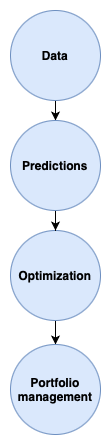
\includegraphics[width=0.2\columnwidth]{Pics/Overview_tree.png}
	\caption{Overview of the project components}
	\label{fig:overview} % Should be placed after the caption!
\end{figure}

A detailed layout of the system can be seen in figure \ref{fig:tree_future}. With the four steps in figure \ref{fig:overview} in mind, the data collection section is either fetched from simulated or real data. Naturally, the real data is cleaned as described above. Next, the prediction part of the model can be split up into estimated risk and expected returns. The risk is estimated with either SCM or Ledoit and Wolf and the expected return is split up into simple moving average (SMA), exponential moving average (EMA) or LSTM. Furthermore, the calculated expected returns and estimated risks are sent to the optimization loop where the allocation of the stocks, i.e. weights, are calculated for each day. Finally, the data is evaluated with the model quality parameters and the results are printed and plotted.

\section{Implementation}
%skicka in kodsnippar eller pseudokod

\subsection{Data gathering \& cleaning}
The framework is implemented in Python by using data accessible from InvestPy. With Investpy one is given access to Investing.com and their historical stock prices at OMXS30. See details in \ref{fig:DATA_pseud}.

\begin{figure}[h]
	\centering
	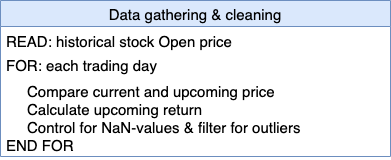
\includegraphics[width=0.7\columnwidth]{Pics/DATA_pseud.png}
	\caption{Pseudocode of Data gathering \& cleaning}
	\label{fig:DATA_pseud} 
\end{figure}

\subsection{Convex optimization solver}

CVXPY is the library in use for solving convex optimization problems. The specified solver used in the project is Mosek since it is more efficient in computation than the standard solver in the CVXPY package.

A pseudocode of the convex optimization solver can be seen in figure \ref{fig:optimization}. The code is split up into two methods. First, the optimization method, which calculates the expected net return for each stock and the risk of the post trade portfolio. By subtracting these values, the convex optimization problem then finds the maximum risk adjusted return for the portfolio by using the library CVXPY and its function \textit{Maximize}.
The second method, \textit{Loop Optimization}, loops the solver over each day. With the results the method calculates the total value of the portfolio, the portfolio's realized return, and the turnover.

%Lägg in källor på biblioteken
%https://www.cvxpy.org/
%https://www.mosek.com/

\begin{figure}[h]
	\centering
	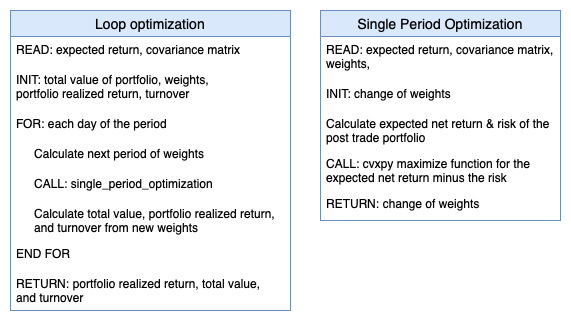
\includegraphics[width=1\columnwidth]{Pics/optimizationPseud.png}
	\caption{Pseudocode of the optimization. Left method is the looping function and right the convex optimization solver.}
	\label{fig:optimization} % Should be placed after the caption!
\end{figure}
\subsection{Predictions}
\subsubsection{SMA \& EMA}
Pseudo-code for implementation of SMA and EMA can be seen in figure \ref{fig:SMAnEMApseud}.

\begin{figure}[h]
	\centering
	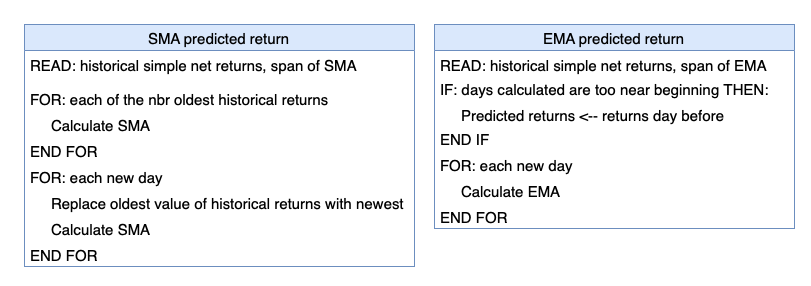
\includegraphics[width=1\columnwidth]{Pics/SMAnEMApseud.png}
	\caption{Pseudocode of the SMA and EMA calculations}
	\label{fig:SMAnEMApseud} % Should be placed after the caption!
\end{figure}
\subsubsection{LSTM} The LSTM model was trained on expected returns between 2010 - 2016. Hyperparameter optimization was done between 2016-2018 and testing was, same as for SMA \& EMA, between 2018-2020.

\subsection{Hyperparameter optimization}
Grid search is used for the hyperparameter optimization meaning that multiple of parameters are tested in conjunction with each other to see which yields the highest SR and lowest TO. For EMA \& SCM different values on $T_{EMA}$ and $T_{SCM}$ are used. As for the risk aversion parameter, varying values of $\gamma$ are tested. The tested values are separated on a logarithmic scale to cover a larger spectrum of potential parameters, see example below. The files are saved as a resulting DataFrame and analysed with the model quality parameters. The data used for the hyperparameter searches were the closing prices of the assets between 2010-2018. 
Since the hyperparamters of the LSTM training are fixed, only a hyperparameter optimization with regards to $\gamma$ and and the estimated risk, for instance $T_{SCM}$ were used. As mentioned, the LSTM training spanned until 2016 so the hyper parameters used for the LSTM predicted returns had to be optimized from 2016 - 2018.

\begin{minted}[fontsize=\tiny]{python}
  
hyperDataFrameEMA = pd.DataFrame(columns=['T_ema','SigmaHyper','Gamma','Turnover',
'SharpeRatio'])

for Tema in np.logspace(3,8, num =5, base=2, dtype='int'):
    for SigmaHyper in np.logspace(1,4,num =4, base=2, dtype='int'):
        for gamma in np.logspace(-1,11,num =7, base=2, dtype='float'): 
            totValueEMA, turnoverEMA, R_Pema, weightsEMA = loop_optimization(
                calcEMA(Tema), 
                covariance_calc_v1, 
                SigmaHyper,
                gamma)
            turnOver, sharpeR = hyperMetrics(totValueEMA, turnoverEMA, R_Pema)
            hyperDataFrameEMA = hyperDataFrameEMA.append({'T_ema': T_ema,
            'SigmaHyper': SigmaHyper, 'Gamma': gamma, 'Turnover': turnOver,
            'SharpeRatio': sharpeR}, ignore_index=True)

hyperDataFrameEMA.to_pickle('./pickle_hyper/hyperDataFrameEMA_SCM.pkl')

\end{minted}


\section{Results}
\subsection{Simulated data}
Using the simulated stock data over a 20 year period with SMA for predicting price changes and the true covariance matrix yielded a portfolio increase from 1 MSEK to 1.05 MSEK over a 20 year period. See figure \ref{fig:GraphtotValues_SMA}. The performance metrics is seen in the table named \textit{SMA Predicted Return} below.

\begin{center}
 \begin{tabular}{||l l||} 
 \hline
 \textbf{SMA predicted return} & \\ [0.5ex] 
 \hline
 Performance metric & Value\\ [0.5ex] 
 \hline\hline
 Total value & $=1050350$ SEK \\ 
 \hline
 Average turnover& $=217.3886$ \\
 \hline
 Realized Sharpe ratio & $=0.072$ \\  [1ex] 
 \hline
\end{tabular}
\end{center}
\begin{figure}[h]
	\centering
	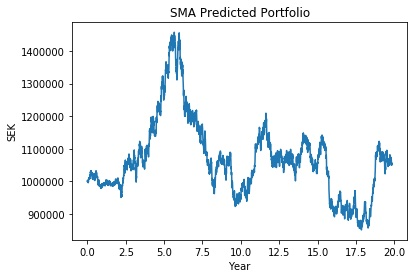
\includegraphics[width=0.8\columnwidth]{Pics/GraphtotValues_SMA.jpg}
	\caption{Total value of portfolio, using SMA predicted returns, over 20 years of simulated stock data.}
	\label{fig:GraphtotValues_SMA} 
\end{figure}
\subsection{OMXS30 Results}
All the results below are from the best performing parameters from the hyperparameter optimization from the years 2018 to 2020 on OMXS30. The models are in the following order: SMA and SCM, EMA and SCM, SMA and Ledoit \& Wolf, EMA and Ledoit \& Wolf, LSTM and SCM and lastly LSTM and Ledoit \& Wolf.

\begin{center}
 \begin{tabular}{||l l||} 
 \hline
 \textbf{SMA \& SCM  model} & \\ [0.5ex] 
 \hline
 Performance metric & Value\\ [0.5ex] 
 \hline\hline
 Total value & $=886870$ SEK \\ 
 \hline
 Average turnover& $=81.3220$ \\
 \hline
 Realized Sharpe ratio & $=-0.323$ \\  [1ex] 
 \hline
\end{tabular}
\label{tab:SMA and SCM data}
\end{center}
\begin{figure}[h]
	\centering
	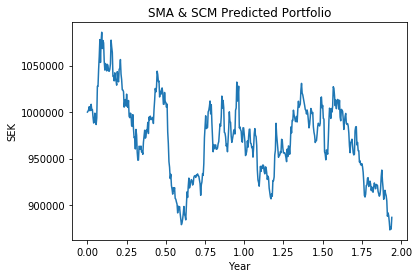
\includegraphics[width=0.8\columnwidth]{Pics/result/SMA_SCM.png}
	\caption{Total value of portfolio, using SMA predicted returns and SCM estimated risk on OMXS30. Timespan is from 2018 to 2020. Hyperparameters in use: SMA: $T_{SMA} =32$, SCM: $T_{SCM} = 8$, risk aversion parameter:$\gamma= 512$}
	\label{fig:SMASCM} 
\end{figure}
\begin{center}
 \begin{tabular}{||l l||} 
 \hline
 \textbf{EMA \& SCM  model} & \\ [0.5ex] 
 \hline
 Performance metric & Value\\ [0.5ex] 
 \hline\hline
 Total value & $=1046026$ SEK \\ 
 \hline
 Average turnover& $=81.9789$ \\
 \hline
 Realized Sharpe ratio & $=0.225$ \\  [1ex] 
 \hline
\end{tabular}
\label{tab:EMA and SCM data}
\end{center}
\begin{figure}[h]
	\centering
	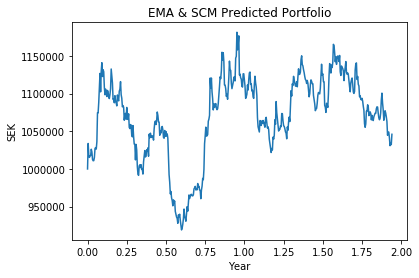
\includegraphics[width=0.8\columnwidth]{Pics/result/EMA_SCM.png}
	\caption{Total value of portfolio, using EMA predicted returns and SCM estimated risk on OMXS30. Timespan is from 2018 to 2020.Hyperparameters in use: EMA: $T_{EMA} =8$, SCM: $T_{SCM} = 8$, risk aversion parameter:$\gamma= 2$}
	\label{fig:EMASCM} 
\end{figure}

%% agges tabeller o grafer


\begin{center}
 \begin{tabular}{||l l||} 
 \hline
 \textbf{SMA \& LW  model} & \\ [0.5ex] 
 \hline
 Performance metric & value\\ [0.5ex] 
 \hline\hline
 Total value & $=894220$ SEK \\ 
 \hline
 Average turnover& $=18.180805$ \\
 \hline
 Realized Sharpe ratio & $=-0.213691$ \\  [1ex] 
 \hline
\end{tabular}
\label{tab:SMA and LW data}
\end{center}

\begin{figure}[h]
	\centering
	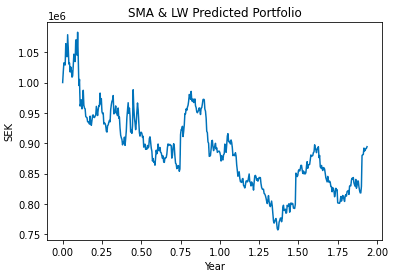
\includegraphics[width=0.8\columnwidth]{Pics/result/SMA_LW_Diagram.png}
	\caption{Total value of portfolio, using SMA predicted returns and LW estimated risk on OMXS30. Timespan is from 2018 to 2020. Hyperparameters in use: SMA: $T_{SMA}$ = 256, LW: Assume Centered = True, risk aversion parameter: $\gamma$ = 0.5}
	\label{fig:SMALW} 
\end{figure}

\begin{center}
 \begin{tabular}{||l l||} 
 \hline
 \textbf{EMA \& LW  model} & \\ [0.5ex] 
 \hline
 Performance metric & Value\\ [0.5ex] 
 \hline\hline
 Total value & $=840567$ SEK \\ 
 \hline
 Average turnover& $=4.19766$ \\
 \hline
 Realized Sharpe ratio & $=-0.544095$ \\  [1ex] 
 \hline
\end{tabular}
\label{tab:EMA and LW data}
\end{center}

\begin{figure}[h!]
	\centering
	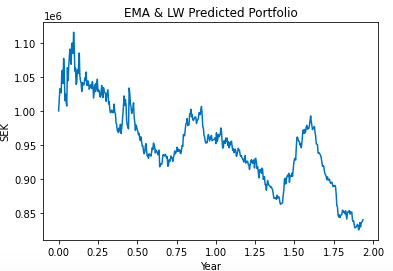
\includegraphics[width=0.8\columnwidth]{Pics/result/EMA_LW_Diagram.png}
	\caption{Total value of portfolio, using EMA predicted returns and LW estimated risk on OMXS30. Timespan is from 2018 to 2020. Hyperparameters in use EMA: $T_{EMA}$ = 8, LW: Assume Centered = True, risk aversion parameter: $\gamma$ = 0.5}
	\label{fig:EMALW} 
\end{figure}

\newpage

\begin{center}
 \begin{tabular}{||l l||} 
 \hline
 \textbf{LSTM \& SCM  model} & \\ [0.5ex] 
 \hline
 Performance metric & Value\\ [0.5ex] 
 \hline\hline
 Total value & $=1135855$ SEK \\ 
 \hline
 Average turnover& $=67.7153$ \\
 \hline
 Realized Sharpe ratio & $=0.5058$ \\  [1ex] 
 \hline
\end{tabular}
\label{tab:EMA and LW data}
\end{center}

\begin{figure}[H]
	\centering
	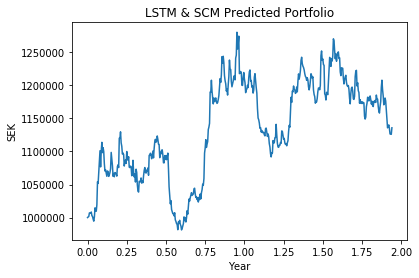
\includegraphics[width=0.8\columnwidth]{Pics/result/LSTM_SCM.png}
	\caption{Total value of portfolio, using LSTM predicted returns and SCM estimated risk on OMXS30. Timespan is from 2018 to 2020.Hyperparameters in use: LSTM: fixed, SCM: $T_{SCM} = 8$, risk aversion parameter:$\gamma= 512$}
	\label{fig:LSTMSCM} 
\end{figure}

\begin{center}
 \begin{tabular}{||l l||} 
 \hline
 \textbf{LSTM and Ledoit \& Wolf model} & \\ [0.5ex] 
 \hline
 Performance metric & Value\\ [0.5ex] 
 \hline\hline
 Total value & $=1081810$ SEK \\ 
 \hline
 Average turnover& $=23.2576$ \\
 \hline
 Realized Sharpe ratio & $=0.3372$ \\  [1ex] 
 \hline
\end{tabular}
\label{tab:LSTM and LW data}
\end{center}

\begin{figure}[h]
	\centering
	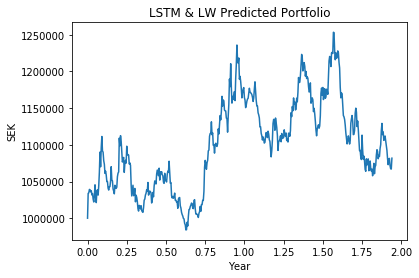
\includegraphics[width=0.8\columnwidth]{Pics/result/LSTM_LW.png}
	\caption{Total value of portfolio, using LSTM predicted returns and Ledoit \& Wolf estimated risk on OMXS30. Timespan is from 2018 to 2020. Hyperparameters in use: LSTM: fixed, LW: Assume Centered $=$ True, risk aversion parameter:$\gamma= 8$}
	\label{fig:LSTMLW} 
\end{figure}

\section{Discussion}
\subsection{Initial challenges}
Before the group felt comfortable working with the framework set up by Boyd et. al (2007) further reading within fundamentals of finance and knowledge in stock trading was needed. Working with convex optimization for optimizing the portfolio also required some further studies of the subject. 

Initially Yfinance was planned to be used as the data gathering API for gathering information related to stock price, but due to unstable results and frequent crashes of the program, caused by the API, the group decided to go with Investpy instead.

\subsection{Summary}

Examining the results, the LSTM models performed the best. The LSTM and Ledoit \& Wolf model got the lowest average turnover, $2326\%$, with a positive sharpe ratio. However, with an estimated brokerage fees of $0.5\%$ that turnover would result in fees equivalent to $0.005\cdot 1000000\cdot23.26 = 116300 $ SEK and there would not be any direct profit. 

Since trading cost was not a constraint in the optimization method it is not particularly odd to see such high values on the average turnover for each and every model. In general one can see a lower turnover rate in the cases when the covariance matrix is used as formulated by Ledoit \& Wolf in comparison to the SCM. Reasons to this may be due to the fact that the extreme coefficients are pulled towards the center values when using LW to reduce estimation errors whereas SCM is more static and error prone since it is just more or less a rolling average. One cannot based on this result directly tell what statistic model perform the best since they perform differently based on what estimated risk parameter they are combined with. 

\subsection{Potential improvements}
As previously mentioned, the missing values are removed from the dataset. Consequently, a day worth of information is lost. An improvement would be to use several data sources and add the missing information from one to another. This could also mean that one could analyse the supplied data more sceptical in order to see if it lacked real data.

Implementing a model for calculting trading cost would be beneficial for the optimization and redistribution of stocks. This would result in a lower turnover and consequently lower the total loss of profit due to brokerage fees.

The hyperparameter optimization could be more thorough for the different models. Given more time and computational power one could have done grid searches with even more values and hopefully found even more optimized hyperparameters. Another alternative is to use bayesian optimization to find the best hyperparameters. Bayesian optimization is more time-efficient than grid searching when working with smaller input ranges in a black box environment.\cite{ref:Bayesian}

Looking at the LSTM predicted returns, an improvement would be to go back as far as possible for each of the models generated for the stocks. This would mean back to the 1980s for some stocks. In addition, doing an hyperoptimization of the NN parameters could also have resulted in a better model. However, the issue of computing power arises so maybe some sort of cloud based computation would be needed.

Different learning methods besides LSTM could be implemented as well in order to get even more precision on the returns. 

Once the predictions for Single-Period Optimisation are deemed stable, Multi-Period Optimisation could be implemented in order to create a portfolio which can re-balance it's assets not only on how it predicts the returns \& risk to change from one trading day to another, but through further predictions into multiple trading days into the future


\section{Appendix A}
\begin{figure}[h]
\centering
	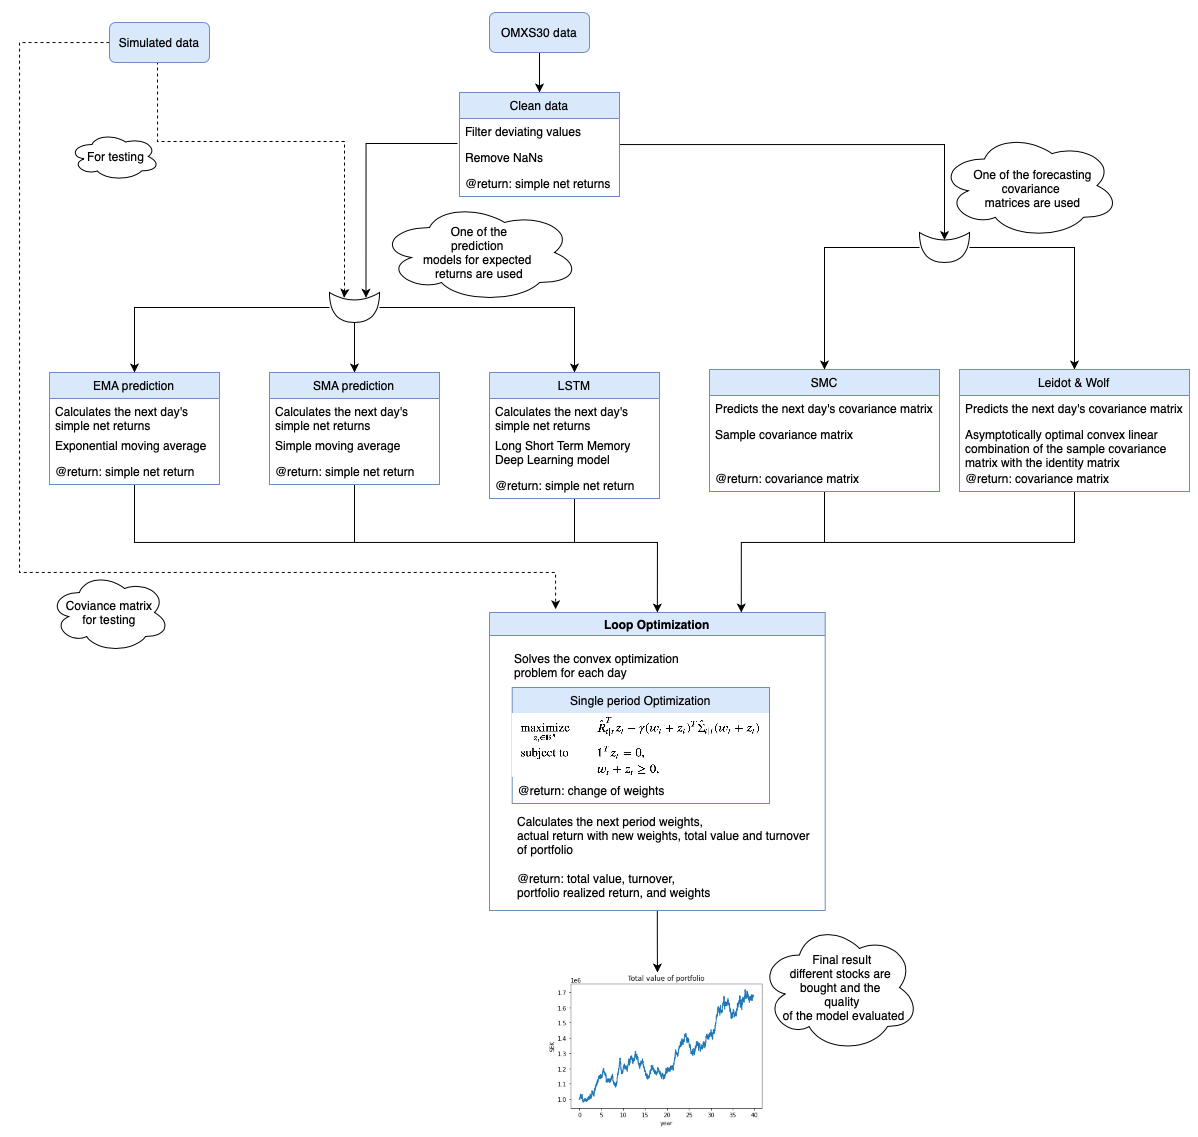
\includegraphics[width=0.5\textwidth]{Pics/Mod_overview_future.png}
	\begin{centering}
	\caption{Tree overview of the project methods. Right hand side of the figure shows the future work including other prediction for expected returns. The covariance matrix needs to be estimated and the real data will be used}
	\label{fig:tree_future}
	\end{centering}
	 % Should be placed after the caption!
\end{figure}






% Prints cited references

\printbibliography [b]


\end{document}


